\section{Calorimeter}

A primary goal of the CLAS12 physics program is to study internal dynamics of the nucleon . 
These experiments require accurate kinematical analysis of neutral and charged particles at high momentum. 
In particular, all CLAS12 electro-production experiments require the efficient detection and reliable identification 
of energetic electrons, photons, and neutrons using the forward electromagnetic calorimeter (ECAL).

One of the primary usages of ECAL system is separating electrons from other particles, like pions, using 
energy deposited in the calorimeters. To accommodate hexagonal design of CLAS12 detector ECAL is using 
triangular hodoscope layout. The scintillating layers have three alternating stereo readout planes named U,V and W, 
which are interleaved with layers of lead as shown on Figure~\ref{clas12:ecal}

\begin{figure}[!ht]
\begin{center}
 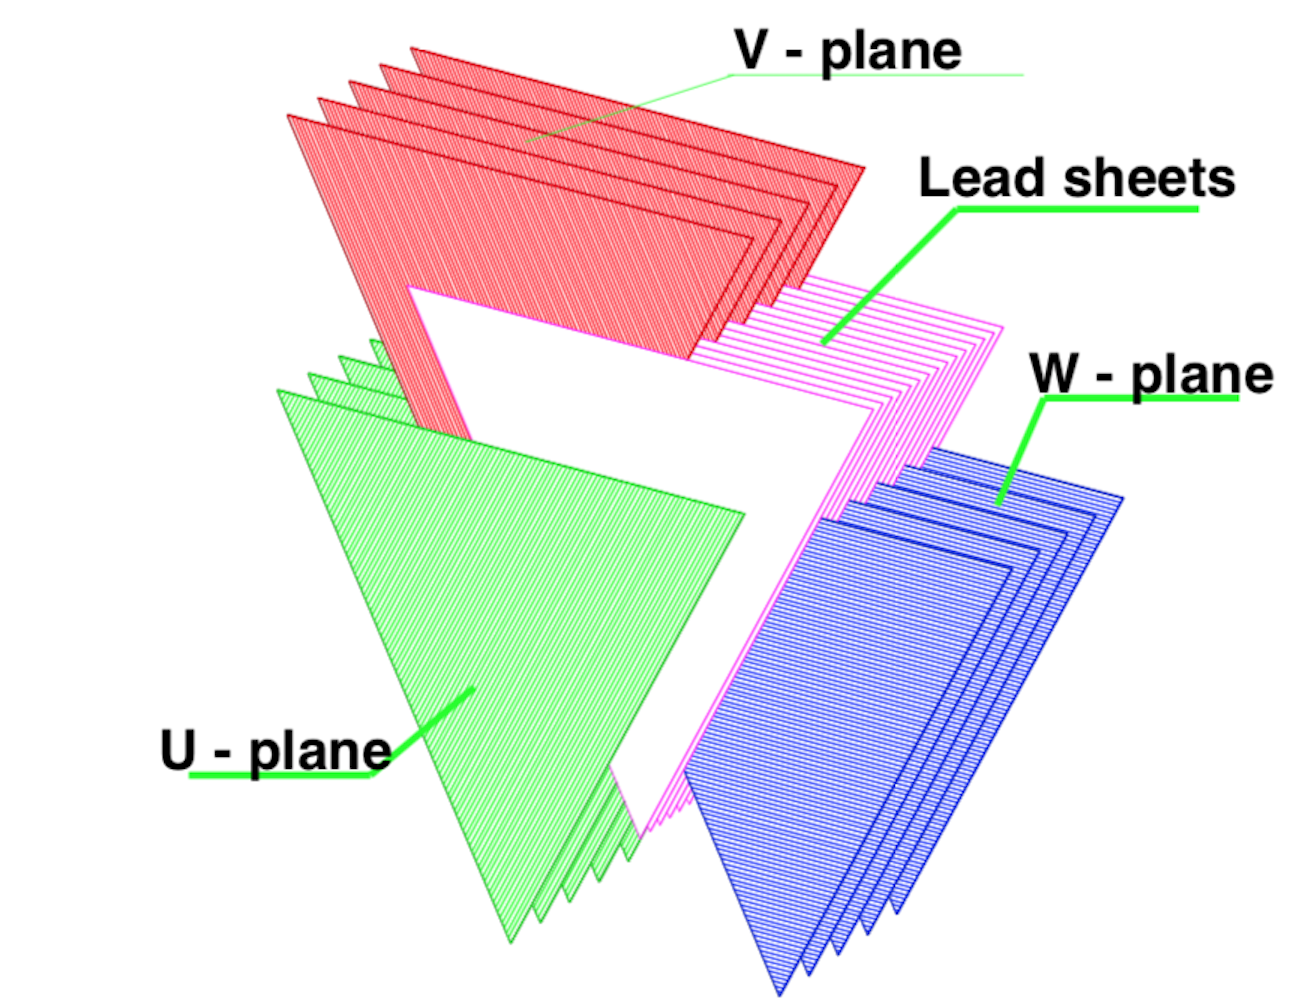
\includegraphics[width=3.in]{images/calorimeter_layers.png}
 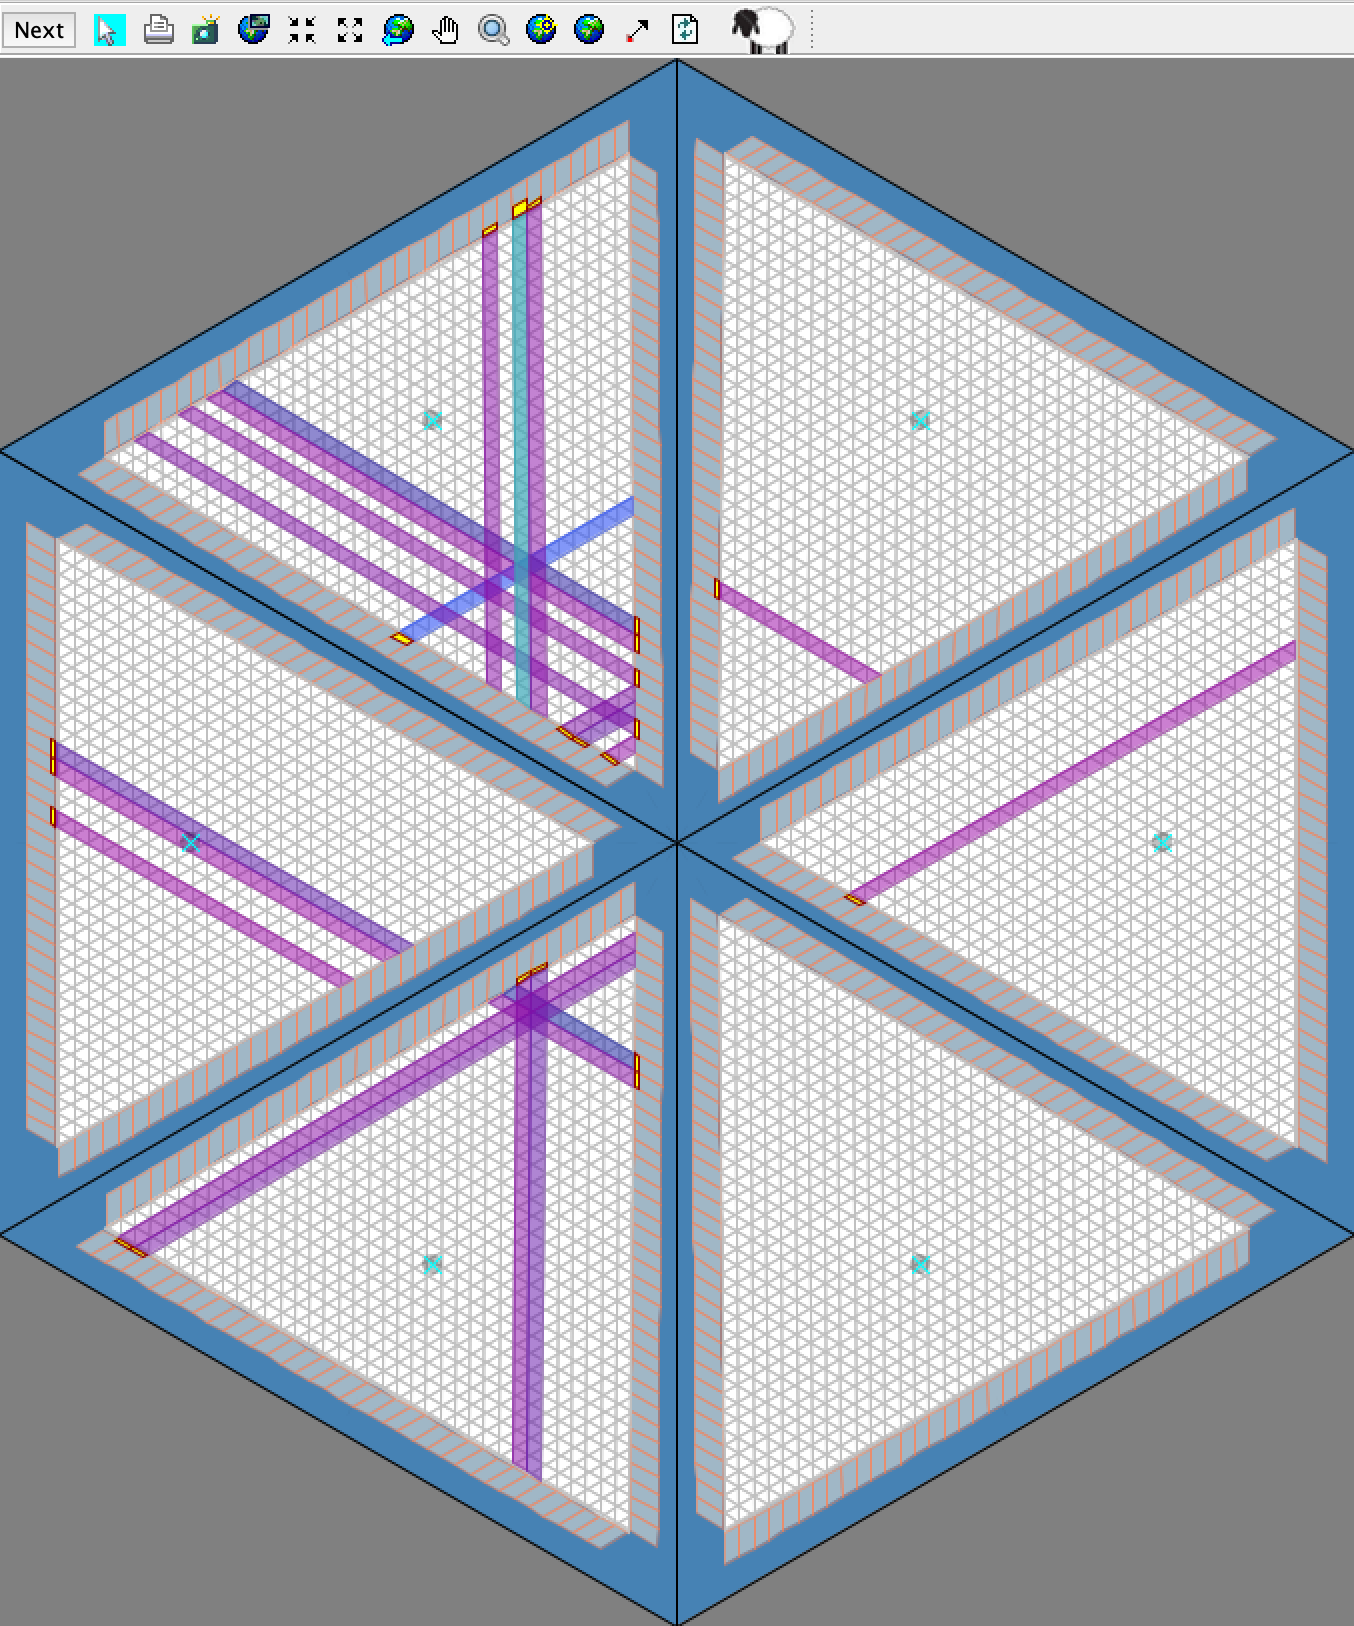
\includegraphics[width=2in]{images/ecal_view.png}
\caption { CLAS12 Electromagnetic Calorimeter structure description.}
 \label{clas12:ecal}
 \end{center}
\end{figure}

When particle enters the calorimeter it leaves signal in each of the layers (U,V and W), and is readout independently.
For each layer a cluster (called peak) is constructed by grouping adjacent hit strips and peaks from all three sides are combined into a cluster if they intersect in one point on the surface. A typical cluster is shown on Figure~\ref{clas12:ecal}.
